\documentclass[11pt]{article}
\usepackage{cite}
\usepackage{url}
\usepackage{amsthm}
\usepackage{amsmath}
\usepackage{amsfonts}
\usepackage{setspace}
\usepackage[toc,page]{appendix}
\usepackage{float}
\usepackage[pdftex]{graphicx}
\theoremstyle{plain}
\newtheorem{theorem}{Theorem}[section]
\newtheorem{corollary}[theorem]{Corollary}
\newtheorem{definition}[theorem]{Definition}
\newtheorem{lemma}[theorem]{Lemma}
\newtheorem{proposition}[theorem]{Proposition}
\newtheorem{example}[theorem]{Example}
\title{NA}
\author{NA}


\begin{document}

\begin{abstract}
We present a basic axiomatization for the discrete case of the
concept of entropy by using a minimum amount of axioms. This
axiomatization is satisfied by most of the entropies that are
known in the literature, as for instance Shannon's, Renyi's,
Varma's, etc. We analyze also the mathematical consequences of
these axioms from a topological and functional point of view. This
analysis leads us to the conclusion that entropies live in a non
compact convex subset of the Banach space $C(\Delta_{n})$ with the sup norm.
Finally, we prove that there exist as many different families of
entropies as real numbers. A result with immediate relevance in different fields of knowledge, ranging from statistics to engineering.

\end{abstract}
%\begin{keyword}
%\end{keyword}
%%PACS:


%%%%%%%%%%%%%%%%%%%%%%%%%%%%%%%%%%%%%%%%%%%%%%%%%%%%%%%%%%%%%%%%%%%%%%%%%%%%%%%%%%%%%%%%%%%%%%%%%%%%%%%%%%%%%%%%%%
%%%%%%%%%%%%%%%%%%%%%%%%%%%%%%%%%%%%%%%%%%%%%%%%%%%%%%%%%%%%%%%%%%%%%%%%%%%%%%%%%%%%%%%%%%%%%%%%%%%%%%%%%%%%%%%%%%
\section{Introduction}
In 1948 C. Shannon \cite{Shannon} introduced the concept of
information theoretic entropy, defined by the formula
\begin{equation}
H(p_{1},\ldots,p_{n})=-\sum_{i=1}^{n} p_{i}\ln(p_{i}).
\end{equation}
\\
The importance of this entropy goes beyond the original scope that
C.Shannon intended when he introduced it. In 1957 the physicist E.
Jaynes introduced a new technique to find prior probabilities in
Bayesian Statstics \cite{Jaynesfull, Gregory, sivia}. The idea was
to maximize Shannon's entropy subject to different constraints.
According to Jaynes the maximization of entropy principle
(MEP) ought to be the best way to find prior probabilities whatever
testable information we have at hand. This, despite the fact that
Shannon's entropy is not the unique way to measure information
content. In Jaynes' words \cite{Jaynes3, Inadequacy}
\begin{quotation}
"One...Important reason for preferring the  Shannon measure of
information is the only one that satisfies...[Shannon's
postulates]. Therefore one expects that any deduction made from
other information measures, if carried far enough, will eventually
lead to a contradiction".
\end{quotation}

Time has shown that no such contraditcion arrives, in fact, uses
of other information measure proves to be very valuable when
studying different types of systems. For example in statistical
mechanics we have the concept of Tsally's entropy \cite{Tsallis2,
Tsallis3,Tsallis1, Gellmann}. Also a bunch of all other entropies
have found their applications in areas very far from physics, like
in Image analysis \cite{Kappur}.
\\
The previous discussion gives an idea of the relevance that a solid axiomatization of the concept of entropy  would have in several branches of knowledge. This relevance is the reason why several attempts have been made to  give an axiomatic foundation to the theory of entropies. These different axiomatic approaches can be found elsewhere \cite{Ochs,Csizar, Characterizing, Aczel} . 
\medskip
\\
The way the axioms are chosen in order the develop the theory is a matter of taste, as long as most of the known entropy-like  functions fulfill this
axioms, and these axioms reflect what we intuitively understand as information. 
\\
The aim of this paper is to give a cogent axiomatic foundation for
the theory of discrete entropies, trying to put as little axioms as possible. After this, we  explore the consequences that the set of chosen  axioms have,  from the mathematical point of view and from the applications point of view.
\medskip
\\
The difference between this paper and other papers that axiomatize
entropies as well (e.g. \cite{Dupuis, Csizar}) is that in this work, the
number of axioms is kept to a minimum, therefore obtaining more
general results. Results that are applicable to a wider range and
are more fundamental.
\medskip
\\
This papers goes as follows:  Section 2 Presents a brief discussion on what do we mean by an information measure; Section 3 presents a brief summary of some well known generalized entropies; In section 4 we develop the consequences
of the axiomatization, where the main results are presented;
Finally section 5 shows the analysis and conclusions of the results obtained.


\section{What does an information measure mean?}
To illustrate what we mean by an information measure, consider the following example: Someone throws a dice, of course, if we knew the initial conditions when the die was thrown, we can use Newton's second law to predict the outcome of the dice. However knowing all the information necessary to predict the outcome  is practically impossible, therefore we cannot say for sure which of the numbers from $1$ to $6$  is going to be shown by the dice. An smarter approach could be the following: Assign a  probability $\{p_{1},p_{2},\ldots,p_{6}\}$ to each  of the possible outcomes, using the 'information' we have about the system. The key question is. How can we  assign the probabilities to the different outcomes, based on what we know?  We can argue that there must be a way to assign probabilities based on what we know about the system. For example if we know nothing about the system and the initial conditions of the dice prior to be thrown, then, our intuition tells us that the logical thing to do is to assign equal probabilities to each of the outcomes i.e. $p_{1}=\frac{1}{6},\ldots,p_{6}=\frac{1}{6}$. A more complicated scenario is when you know that the die is charged, say towards $4$. Clearly in this case equal a prior probabilities doesn't seem to be the right way to go, but some probability distribution centered at $4$. 
\medskip
\\
In the previous situation one may ask. Assuming that there is a way to assign probabilities that reflects our state of knowledge about the system, is there any systematic way to assign those probabilities? Here is where the concept of information measure comes into play. In our previous example assume that there exists a bounded function $f$ of the probabilities assigned, such that for each probability distribution $\{p_{1},\ldots,p_{6}\}$ assigns a non negative  real number , i.e. $f(p_{1},\ldots,p_{6})\in\mathbf{R^{+}}$. If that number were a quantitative representation of how much we know about the system, then, we can arbitrarily assign the number $0$ to total knowledge (i.e we know the outcome before throwing the dice) and the number $\sup_{x} f(x)$ to total ignorance (i.e. we don't know anything about the system).  A function with the characteristics described above, can be considered as an information measure.
\medskip
\\
Our goal in this paper is to find the biggest set of functions that can be considered as information measures.To do that we first propose the set of axioms that we consider that must be fulfilled by an information measure. After that, we are going to explain the intuition behind those axioms, and the practical applications that those axioms have.

\subsection*{Axioms}
We are going to start this discussion from a purely mathematical point of view and then we are going to put things down to earth.
\newline
\\
For any $n \in  \mathbb{N}$ , define the \textbf{continuous} function
\begin{equation}
\tilde{S}:\Delta_{n}\subset \mathbb{R}^n\rightarrow \mathbb{R},
\end{equation}
where
\begin{center}
$\Delta_{n} =\{(p_{1},\ldots,p_{n})\in\mathbb{R}^n|\sum_{i=1}^{n}
p_{i}=1, p_{i}\geq 0\}.$
\end{center}

Clearly the points in the domain of the function $\tilde{S}$ can
be regarded as probabilities of a set of exhaustive events. Also
it is worth noticing that this domain is nothing more than the
n-simplex from algebraic topology.
\medskip
\\
We want the function $\tilde{S}$ to satisfy the following axioms

\begin{enumerate}
\item Given $\sigma \in P_{n}$ where $P_{n}$ is the permutation group of
a set with $n$ elements. Let
$x=(p_{1},\ldots,p_{n})\in\Delta_{n}$ then $\tilde{S}$ satisfies
permutation of its arguments invariance, that is,
$\tilde{S}(x)=\tilde{S}(\sigma(x))$ where
$\sigma(x)=\sigma(p_{1},\ldots,p_{n})=(p_{\sigma(1)},\ldots,p_{\sigma(n)})$.
\item Given x $\in\Delta_{n-1}$, then $\tilde{S}(x)=\tilde{S}(x,0)$.
\item Define $u_{k}=(\frac{1}{k},\ldots,\frac{1}{k})\in\Delta_{k}$, then if
$m,n$ $\in\mathbb{N}$ with $m \leq n$, we have
$\tilde{S}(u_{m})\leq\tilde{S}(u_{n})$. Also
$\tilde{S}(x)\leq\tilde{S}(u_{n})$ for all $x\in\Delta_{n}$.
\item $\tilde{S}(x)=0$ if and only if x is one of the canonical base vectors
 of $\mathbb{R}^n$.
\end{enumerate}

This four axiom are intended to reflect the minimum properties
that are expected for an information measure. Lets do a little digression on the idea that every axiom is trying to convey. 
\newline
\\
Axiom 1,says that the only thing that matters in the entropy function is the
probabilities per se, not which probability gets each of the event
whose probability is being measured.This is reasonable, because  for example suppose that we like to
measure our uncertainty about a coin toss and is known that the
probability of head is 0.3 and tail 0.7, we have the same amount
of information if we know that the probability of head is 0.7 and
of tail 0.3. 
\newline
\\
Axiom 2 tells  that if in a set of events is included
one event with probability 0 our state of knowledge remains the
same.
\newline
\\
Axiom 3 states the fact that equal probabilities for
exhaustive events is the most ignorant we can be about something
and the more  events, the more ignorant we are. 
\newline
\\
Finally axiom 4
just says that if we have an event with probability 1 (implying
that the probabilities of the other events are  0). We know before
hand  the outcome so we are not ignorant at all.\medskip
\newline
\\
It is worth noticing that we asked the function $\tilde{S}$ to be continuous. The reason for this is the following. If the probabilities of an event change little then our state of knowledge represented by $\tilde{S}$, also changes little. This is the intuitive meaning of continuity.
\medskip
\\
Now that we stated what we want, we need to check how useful it is. To do so, we are going to review some of the well known discrete entropies that exists in the literature.




\section{A brief Review on generalized entropies}
To put ideas into context it is necessary to review a few of well
known generalized entropies and check if they satisfy the axioms proposed in the previous section. It is an straightforward exercise to check that the axioms are fulfilled by each of the functions that we are going to present, therefore we only going to present the functional form of this entropies.

\subsection*{Tsallis Entropy}
One of the most famous attempts to generalize Shannon's entropy
was made by the Brazilian Physicist Constantino Tsallis, with the
so-called Tsallis entropy \cite{Tsallis2}.
\begin{equation}
S(p_{1},\ldots,p_{n})=\frac{1-\sum_{i=1}^{n} p_{i}^{q}}{q-1}
\end{equation}
It is a generalization of Shannon's entropy in the sense that when
the parameter $q$ goes to 1, Tsallis entropy becomes Shannon's
entropy.

\subsection*{Renyi's Entropy}
Another famous generalization is Renyi's entropy \cite{Renyi},
which has wide application in many areas of mathematics.
\begin{equation}
H_{\alpha}(p_{1},\ldots,p_{n})=\frac{1}{1-\alpha}\ln(\sum_{i=1}^{n}
p_{k}^{\alpha})
\end{equation}

\subsection*{Varma and Kapur}
There are also some generalizations of Renyi's entropy of order
$\alpha$\cite{Varma, Kappur2}.

\begin{equation}
\frac{\ln(\sum_{i=1}^{n} p_{i}^{r-m+1})}{m-r}, m-1<r<m, m\geq 1,
\end{equation}
\begin{equation}
\frac{\ln(\sum_{i=1}^{n} p_{i}^{\frac{r}{m}})}{m(m-r)}, 0<r<m,
m\geq 1.
\end{equation}
\begin{equation}
\frac{ln(\frac{\sum_{i=1}^{n} p_{i}^{t+s-1}}{\sum_{i=1}^{n}
p_{i}^{s}})}{1-t}, t\neq 1, t>0, s\geq 1.
\end{equation}

\subsection*{Non-additive Measures}
In statistical mechanics the concept of entropy satisfies
additivity, however some systems does not satistfy this additivity
condition, hence are called non-additive systems \cite{Tsallis1}.
Therefore entropies that are non-additive are of great importance,
like the following ones \cite{Sharma, Picard}.

\begin{equation}
-2^{r-1}\sum_{i=1}^{n} p_{i}^{r}\ln(p_{i}), r>0,
\end{equation}
\begin{equation}
\frac{\sum_{i=1}^{n} p_{i}^{r}-p_{i}^{s}}{2^{1-r}-2^{1-s}}, r\neq
s,r>0, s>0,
\end{equation}
\begin{equation}\
-2^{1-r}\frac{\sum_{i=1}^{n} p_{i}^{r}sin(\ln(p_{i}))}{sin(s)}.
\end{equation}

\begin{equation}
-\frac{\sum_{i=1}^{n} v_{i}\ln(p_{i})}{\sum_{i=1}^{n} v_{i}},
\end{equation}
\begin{equation}
\frac{ln(\frac{\sum_{i=1}^{n} p_{i}^{r-1}v_{i}}{\sum_{i=1}^{n}
v_{i}})}{1-t}, s\neq 1, s>0,
\end{equation}
\begin{equation}
\frac{(\exp((s-1)\sum_{i=1}^{n} v_{i}\ln(p_{i}))/\sum_{i=1}^{n}
v_{i}}{2^{s-1}-1}, s\neq 1, s>0,
\end{equation}
\begin{equation}
\frac{((\sum_{i=1}^{n} p_{i}^{r-1}v_{i})/\sum_{i=1}^{n}
v_{i})^{\frac{s-1}{r-1}}-1}{2^{s-1}-1}, r\neq 1, s\neq 1, r>0,
s>0.
\end{equation}

\medskip

These are only a few of the generalized entropies that exists in today's literature where as far as we know there exists more than 20 of those.

Now that we have checked that our axiomatization is useful in the entropy world, it is time to explore the consequences of those axioms. This is going to be done next.






\section{Mathematical consecuences of the axiomatization}

Before  the main results are presented,it is necessary to do some
mathematical preliminaries, in order to put ideas in a more clear
language.

\begin{definition}\label{thm:equivalence}
Let $x,y$ $\in\Delta_{n}$, for any n $\in\mathbb{N}$, we say that
$x$ is equivalent to $y$ ($x\sim y$) if and only if $x=\sigma(y)$ for
some $\sigma\in P_{n}$. 
\end{definition}
It is straightforward to check that $\sim $ is an equivalence relation over $\Delta_{n}$. Now we are going to state a lemma an a definition that will serve as a basis for a new construction over the information measure $\tilde{S}$.

\begin{lemma}
Let $x=(p_{1},\ldots,p_{n}) \in\Delta_{n}$ such that
$p_{i_{1}}=p_{i_{2}}=\ldots=p_{i_{k}}=0$ for $k<n$ then there
exists  $\sigma\in P_{n}$ such that the last $k$ entries of
$\sigma(x)$ are 0.
\end{lemma}

%\begin{proof}
%choose $\sigma$ such that $\sigma(i_{k})=n,
%\sigma(i_{k-1})=n-1\ldots \sigma(i_{1})=n-k$ and 0 the other
%indices elsewhere. From this is clear that the vector $\sigma(x)$
%has the first n-k entries different from 0 and the last k entries
%are 0's.
%\end{proof}


\begin{definition}\label{def:D}
Given the equivalence relation $\sim$ on $\Delta_{n}$. We call $D_{n}$ the
quotient set $\Delta_{n}/\sim$.
\end{definition}


The last lemma and definition shows that without lost of
generality, if a vector  $x\in \Delta_{n}$ has $k$ 0's in it. Is safe
to assume that they are in the last $k$ entries (this vector is the
class representative of the equivalence class of $x$).\smallskip
\\
Now we are ready to define a more concrete mathematical element that can be regarded as a true information measure.

\begin{definition}
We define the function  $S:D_{n}\rightarrow\mathbb{R}$, by the relation
$S([x])=\tilde{S}(x)$, where $[x]$ is the equivalence class of x
by the equivalence relation $\sim$.
\end{definition}

There is a very powerful reason to define the new function $S$,
besides the fact that it is easy to work with class equivalences.
In the four axioms, nothing was said about how the entropy must
behave when measuring uncertainity on conjunction of independent
events. For example if there are 3 independent events $A_{1},
A_{2}, A_{3}$ with probabilities $p_{1},p_{2}, p_{3}$. then one of
the possible vector containing the values of the probabilities of
the conjuntion of all the events is
$(p_{1}p_{2},p_{1}p_{3},p_{2}p_{3})$. But the vector
$(p_{2}p_{3},p_{1}p_{3},p_{1}p_{2})$ has the same information
about all the conjunction of the 3 events. Thanks to the
definition of $S$ there is no need to worry about which vector to
use. So, this facilitates future studies on axiomatization of
entropies and how they behave under composition of diferent
events.
\newline
\\
With the new domain of definition $D_{n}$, it is necessary to see
which properties of the set $\Delta_{n}$ are inherited by the
quotient set $D_{n}=\Delta_{n}/\sim$. To study this, first a topology must
be define
 on the quotient set. The natural way to do this is by
giving $\Delta_{n}/R$ the finest topology that makes the canonical
projection function continuous \cite{Rubiano, Janich}. Here is used
the universal convention to denote the canonical projection by the
letter $\pi$ . The  topology generated by $\pi$ is called the quotient topology. From
the topological properties of continuous function, is concluded
that because $\Delta_{n}$ is a closed, bounded set on
$\mathbb{R}^{n}$, then it is compact. Obviously is connected also. Then, since
$D_{n}=\Delta_{n}/\sim$ is the image of $\pi$, is also
compact\footnote{Therefore by the Wierstrass theorem, S, which is
continuous as shown in theorem $\ref{cor:continous}$ attain a
maximum in D. That maximum is reached in the equivalence class of
the vector $u_{n}$. To see this,let [x] $\in$ D,then the following
holds $S([x])=\tilde{S}(x)\leq \tilde{S}(u_{n})=S([u_{n}])$} and
connected. In fact it can be shown that $\Delta_{n}$ is
homeomorphic to $\Delta_{n}/\sim$.

\begin{theorem}
The sets $\Delta_{n}$ and $\Delta_{n}/\sim$ are homeomorphic.
\end{theorem}

\begin{proof}
For the sake of simplicity  consider the case of the 2-simplex
which is just a triangle, as shown in figure 1. The barycenter is
nothing more than the point where all entropies attains their
maximum. Also observe that this is a common point for the
triangles COE,EOB,BOD,DOA, AOF,and FOC . Obviously any probability
vector $(p_{1},p_{2},p_{3})$ belongs to any of this triangles, but
the following is also true: If the vector belongs to COB, for
example, then his 6 permutations belongs each one to a diferent
triangle. Hence all of the triangles contains 1 representative of
each of the equivalent classes. This means that all of the
quotient space can be thought as any of the 6 triangles. Because
any of this triangles has the same dimension of the 2-simplex we
can use the result that given two simplexes they are homeomorphic
if they have the same dimension. Hence the proof is completed.
\end{proof}

\begin{figure}[H]
\centering
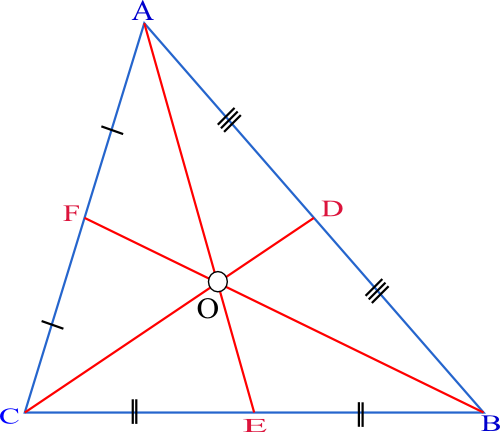
\includegraphics[scale=0.5]{Center}
\caption{2-simplex and its Barycenter}
\end{figure}

This theorem shows that working with $\tilde{S}$ or $S$ is basically
the same thing. But the advantage of working with $S$ instead of
$\tilde{S}$ is that we are working with class equivalences instead of single points in the $n-simplex$. From now on,  no distinction is
going to be made between a vector $x$ and its equivalence class $[x]$. To finish the construction of $S$ we are going to stated the following  key result.


\begin{corollary}\label{cor:continous}
S is continous.
\end{corollary}
\begin{proof}
Since $S=\tilde{S}\circ\pi$, and each of these functions is continuous, the result holds.
\end{proof}

This last corollary along with the result that $D_{n}$ for any $n\in\mathbb{N}$ is compact
guarantee that S also attains its maximum \cite{Zeidlernonlinear}.
So there is  no problem about using  maximization principles on the function $S$.\medskip
\\
Now that   all the mathematical  tools have been developed and the language is clear, we can group all the entropies into one set, this set is defined as follows

\begin{definition}
For any $n \in \mathbb{N}$ we define $X=\{ S:D_{n}\rightarrow
\mathbf{R}|$ S is continuous and satisfies axioms 1 to 4$\}$.
\end{definition}


Since entropies are continuous, X is a subset
of the set of real valued continuous functions on $D_{n}=\Delta_{n}/\sim$,
denoted by $C(D_{n})$. Because the entropy reach its maximum on $D_{n}$, $X$
can be regarded as a subset of the Banach space $C(D_{n})$ with the
sup norm. That is: given $f\in C(D_{n})$, $\|f\|=\max_{x\in D_{n}}
|f(x)|$\cite{rudin}. 
\newline
\\
Whenever we have the objects under study in one particular set, we want to know more about that set, to see if we can get any insights about its structure and hopefully those insights will lead us to some real world applications.

\begin{theorem}\label{thm:notclosed}
The set $X$ is not closed.
\end{theorem}

\begin{proof}
Take the sequence $\{S_{\frac{1}{n}}\}_{n \in \mathbf{N}}$ where
$S_{\frac{1}{n}}$ is the Tsallis entropy
\begin{equation}
S_{\frac{1}{n}}=\frac{1-\sum_{i=1}^{m}
p_{i}^{\frac{1}{n}}}{\frac{1}{n}-1}.
\end{equation}
It is straightforward to see that $\lim_{n \to \infty}
S_{\frac{1}{n}}=m-1$. However, the constant  function $m-1$ does not satisfies
axiom 4. Therefore, exists sequence in X that do not converge in
the set, so X does not contain all of its accumulation points,
hence cannot be closed \cite{Rubiano, Janich}.
\end{proof}


Since every compact set is closed and bounded, we conclude that the following corollary holds.
\begin{corollary}
The set $X$ is not compact.
\end{corollary}


This result makes a little harder future analysis on this set,
because compactness is a desirable property. The reason is that an
infinite compact set behaves very much like a finite one, making
analysis more easy.\medskip
\\
Despite the fact that $X$ is not compact, $X$ has a very nice
topological property.

\begin{theorem}\label{thm:convex}
The set X is convex.
\end{theorem}

\begin{proof}
Let $S_{1},S_{2}\in X$ and let $S(x,t)=(1-t)S_{1}(x)+tS_{2}(x)$,
with $x=(p_{1},\ldots,p_{n})$. Clearly S is invariant under
permutations. Also we have that
$S(x,0,t)=(1-t)S_{1}(x,0)+tS_{2}(x,0)$ and because $S_{1}$ and
$S_{2}$ satisfies axiom 2, we have that
$S(x,0,t)=(1-t)S_{1}(x,0)+tS_{2}(x,0)=(1-t)S_{1}(x)+tS_{2}(x)=S(x,t)$
hence $S(x,t)$ also satisfies axiom 2 for all t. Now let $u_{k}$
be defined as in axiom 3, then if m$\leq$n we have that
$S_{i}(u_{m})\leq S_{i}(u_{n})$ for i=1,2, we have that for $0\leq
t\leq 1$
\begin{equation}
S(u_{m},t)=(1-t)S_{1}(u_{m})+tS_{2}(u_{m})\leq
(1-t)S_{1}(u_{n})+tS_{2}(u_{n})=S(u_{n},t).
\end{equation}
Also is clear that the maximum of $S(x,t)$ is reached when $S_{1}$
and $S_{2}$ are evaluated at the vector $u_{n}$, therefore given
$x\in \Delta_{n}/R$ we have $S(x,t)\leq S(u_{n},t)$.\smallskip
Finally  $(1-t),t,S_{1},S_{2}$ is positive, so we have that if
$S(x,t)=0$ the only posibility is that $S_{1}=0$ and $S_{2}=0$ and
this is true if and only if x is one of the basis vectors of
$\mathbb{R}^{n}$. So we can conclude that $S(x,t)\in X$ for all
$0\leq t\leq 1$. Hence X is convex.
\end{proof}

The fact that $X$ is a convex set allow the following important
result.

\begin{theorem}
There exists at least as much entropies as real numbers.
\end{theorem}

\begin{proof}
The function $\varphi:[0,1]\rightarrow X$ defined by the formula 
\begin{equation}
\varphi(t)= (1-t)S_{1}(x)+tS_{2}(x), 
\end{equation}
for fixed entropies $S_{1}$ and $S_{2}$ is a one to one mapping. Since the cardinal of real numbers is the same as the cardinal of $[0,1]$, we conclude that the cardinal of $X$ is bigger than the cardinal of $[0,1]$.
\end{proof}
Finally since the set of entropies is a subset of the set of continuous functions, a well known result states that the cardinal of the set of real valued functions is the same as the cardinal of the real numbers \cite{Settheory}. Using the previous theorem with this fact we obtain the major mathematical result of this paper.

\begin{theorem}
There exists as much entropies as real numbers.
\end{theorem}

The question that arises now is. What are these results  good for? A first approach to this question will be given in the conclusions section.
\section{Conclusions}

Because only a few axioms were used, the results presented here are
very general and with wide applicability. Also shows that only 4 axioms are needed in order to convey a nice structure of the set of entropies, both from a
topological point of view and  a physical point of view.

To show an idea of how the results presented in this work could be useful outside the realm of mathematics, consider the first  consequence of theorem \ref{thm:convex}. if a set of positive number $\{t_{k}\}_{k=1}^{n}$ are such that $\sum_{k=1}^{n} t_{n}=1$, then for any set of arbitrary entropies $S_{k}\in X$, $k=1,2\ldots n$ we can create a new entropy
\begin{equation}
S=\sum_{k=1}^{n} t_{k}S_{k}.
\end{equation}
The above entropy 'joins' together as many entropies as we want, and the coefficients $\{t_{k}\}$ are the weight on each entropy. Putting this in simple terms, we have created a way to ensemble an entropy that shares features of each of the $S_{k}$ entropies and each feature is as important as the coefficient $t_{k}$.
This have an inmediate application in image thresholding
\cite{Kappur, Matlab} where different types of entropies are used
\cite{renyisthreshold,Tsallisthreshold}, but there exist no
consensus of which entropy is better to maximize in order to
achieve the best thresholding value. With the mixed entropies
proposed in this text it is easy to experiment with different
types of entropies and find out which one is better. 
\smallskip
\\
This argument can also be used in physical systems, so for example we can create a new entropy, based on old entropies, that captures the non reversibility of  the system under study.
\smallskip
\\
One final possible application is in the field of Bayesian statistics, where  the maximum entropy principle is used to choose a objective prior probability distribution. Improving the foundations and understanding on the theory of entropies could enhanced how to find objective a prior probabilities
\newline
\\
The possible applications described above give an idea of how the results obtained in this work can be used to produce results outside the theoretical framework presented here. Although a lot of theoretical work is needed in order to fully explore the consequences that this work brings into the field of entropies.





\newpage


\bibliography{paperBib}
\bibliographystyle{unsrt}


%%%%%%%%%%%%%%%%%%%%%%%%%%%%%%%%%%%%%%%%%%%%%%%%%%%%%%%%%%%%%%%%%%%%%%%%%%%%%%%%%%%%%%%%%%



\end{document}
